\documentclass[11pt,a4paper]{article}

% Packages
\usepackage[utf8]{inputenc}
\usepackage[T1]{fontenc}
\usepackage{amsmath,amssymb,amsthm}
\usepackage{mathtools}
\usepackage{graphicx}
\usepackage{hyperref}
\usepackage{cleveref}
\usepackage{booktabs}
\usepackage{tikz}
\usetikzlibrary{arrows.meta,positioning,shapes.geometric}

% Theorem environments
\newtheorem{theorem}{Theorem}[section]
\newtheorem{lemma}[theorem]{Lemma}
\newtheorem{proposition}[theorem]{Proposition}
\newtheorem{corollary}[theorem]{Corollary}
\newtheorem{definition}[theorem]{Definition}
\newtheorem{remark}[theorem]{Remark}

% Custom commands
\newcommand{\R}{\mathbb{R}}
\newcommand{\C}{\mathbb{C}}
\newcommand{\N}{\mathbb{N}}
\newcommand{\Sp}{\mathrm{Sp}}
\newcommand{\SU}{\mathrm{SU}}
\newcommand{\GPT}{\mathrm{GPT}}

\title{Minimal Axioms for Quantum Structure:\\
What Computation Cannot Derive}

\author{H. Kohashiguchi\\
\small Future Apps Inc.}

\date{December 2024}

\begin{document}

\maketitle

%==============================================================================
\begin{abstract}
%==============================================================================
We investigate the minimal set of axioms required to derive quantum structure from classical computation. Building on our previous work establishing that reversible computation embeds into the classical symplectic group $\Sp(2N,\R)$~\cite{kohashiguchi2024limits}, we employ the framework of Generalized Probabilistic Theories (GPTs) and Resource Theory of Coherence to systematically analyze axiom candidates. Our main results are: (1) \textbf{A1 (state space extension/superposition) is the unique primitive axiom} that cannot be derived from computation; (2) \textbf{information-theoretic principles such as no-cloning are consequences}, not causes, of quantum structure; (3) \textbf{results are universal} across computation models including SK combinatory logic, reversible cellular automata, and lambda calculus. These findings establish clear boundaries on what can be derived from computational substrates and identify the minimal ``quantum leap'' required for quantum mechanics.
\end{abstract}

%==============================================================================
\section{Introduction}
\label{sec:intro}
%==============================================================================

A fundamental question in the foundations of physics and computer science is whether quantum mechanics can be derived from more primitive computational principles. In previous work, we established two key negative results:

\begin{enumerate}
    \item Complex number structure does not automatically emerge from SK combinatory logic~\cite{kohashiguchi2024sk}.
    \item Reversible computation (Toffoli, Fredkin gates) embeds into the classical symplectic group $\Sp(2N,\R)$, not the unitary group~\cite{kohashiguchi2024limits}.
\end{enumerate}

These results demonstrate that computation alone is insufficient for quantum structure, but leave open the question: \emph{What additional axioms are necessary and sufficient?}

In this paper, we address this question using three complementary approaches:
\begin{itemize}
    \item \textbf{Generalized Probabilistic Theories (GPTs)}: A framework for comparing classical and quantum state spaces geometrically.
    \item \textbf{Resource Theory of Coherence}: A framework for treating quantum coherence as a resource, avoiding circular reasoning about no-cloning.
    \item \textbf{Universality verification}: Confirming results across multiple computation models.
\end{itemize}

Our main contribution is the identification of \textbf{A1 (state space extension/superposition)} as the unique primitive axiom for quantum structure. All other quantum properties---including no-cloning, contextuality, and non-commutativity---are derivable consequences.

\subsection{Related Work}

Axiomatic reconstructions of quantum mechanics have been pursued along several lines:
\begin{itemize}
    \item \textbf{Information-theoretic}: Chiribella et al.~\cite{chiribella2011} derived quantum theory from informational axioms including purification.
    \item \textbf{Operational}: Hardy~\cite{hardy2001} proposed five reasonable axioms; Masanes and M\"uller~\cite{masanes2011} used physical requirements.
    \item \textbf{Resource-theoretic}: Coherence as a resource has been formalized by Streltsov et al.~\cite{streltsov2017}.
\end{itemize}

Our work differs in starting from \emph{computation} rather than physics, asking what computation can and cannot provide.

%==============================================================================
\section{Framework}
\label{sec:framework}
%==============================================================================

\subsection{Generalized Probabilistic Theories}

A GPT is defined by a triple $(\Omega, \Sigma, T)$:
\begin{itemize}
    \item $\Omega$: State space (convex set)
    \item $\Sigma$: Effect space (measurements)
    \item $T$: Transformation group
\end{itemize}

\begin{definition}[Classical Computation GPT]
For $n$-bit classical computation:
\begin{align}
    \Omega &= \Delta^{2^n-1} \quad \text{(simplex)} \\
    T &= S_{2^n} \quad \text{(permutation group)}
\end{align}
\end{definition}

\begin{definition}[Quantum GPT]
For $n$-qubit quantum mechanics:
\begin{align}
    \Omega &= \text{Bloch ball (or generalization)} \\
    T &= \SU(2^n)
\end{align}
\end{definition}

The key geometric difference: classical state space is a \textbf{simplex} (discrete extreme points), while quantum state space is a \textbf{ball} (continuous boundary).

\subsection{Axiom Candidates}

We consider six axiom candidates in GPT language:

\begin{enumerate}
    \item[\textbf{A1}] \textbf{State Space Extension}: $\Omega$ is strictly larger than the simplex, with continuous boundary.
    \item[\textbf{A2}] \textbf{Born Rule}: Probabilities are given by inner products.
    \item[\textbf{A3}] \textbf{Reversibility}: Transformations are invertible.
    \item[\textbf{A4}] \textbf{Non-commutativity}: Some measurements do not commute.
    \item[\textbf{A5}] \textbf{No-Cloning}: Universal state copying is impossible.
    \item[\textbf{A6}] \textbf{Contextuality}: Measurement outcomes depend on context.
\end{enumerate}

\begin{remark}[Characterization of A1]
\label{rem:a1-char}
The essential content of A1 is not merely that the state space is ``larger than a simplex,'' but rather that it admits \textbf{transitivity on pure states}: for any two pure states $\psi, \phi \in \partial\Omega$, there exists a continuous reversible transformation $T \in T$ such that $T\psi = \phi$. This transitivity property, combined with reversibility (A3), implies that the state space boundary is a smooth manifold---precisely the Bloch sphere structure of quantum mechanics. This characterization connects our axiom A1 to Hardy's axiom of ``continuous reversibility''~\cite{hardy2001}.
\end{remark}

\subsection{Resource Theory of Coherence}

To avoid circular reasoning about no-cloning (which presupposes non-orthogonal states), we adopt the Resource Theory framework:

\begin{definition}[Coherence Resource Theory]
\begin{itemize}
    \item \textbf{Free states}: Diagonal density matrices (incoherent)
    \item \textbf{Free operations}: Permutations, dephasing, measurements
    \item \textbf{Resource states}: Non-diagonal density matrices (coherent)
\end{itemize}
\end{definition}

The key question becomes: \emph{Can classical computation generate coherence as a resource?}

%==============================================================================
\section{Axiom Analysis}
\label{sec:axioms}
%==============================================================================

\subsection{Axiom Status in Classical vs.\ Quantum}

\begin{table}[ht]
\centering
\caption{Axiom satisfaction by theory type}
\label{tab:axioms}
\begin{tabular}{lccc}
\toprule
Axiom & Classical & Reversible & Quantum \\
\midrule
A1 (State Extension) & \texttimes & \texttimes & \checkmark \\
A2 (Born Rule) & \checkmark & \checkmark & \checkmark \\
A3 (Reversibility) & \texttimes & \checkmark & \checkmark \\
A4 (Non-commutativity) & \texttimes & \texttimes & \checkmark \\
A5 (No-Cloning) & \texttimes & \texttimes & \checkmark \\
A6 (Contextuality) & \texttimes & \texttimes & \checkmark \\
\bottomrule
\end{tabular}
\end{table}

\begin{theorem}[A1 is Primitive]
\label{thm:a1-primitive}
Axiom A1 (state space extension) cannot be derived from A2, A3, A4, A5, or A6.
\end{theorem}

\begin{proof}
Reversible classical computation satisfies A2 and A3 but not A1. This provides a counterexample: A2 $\land$ A3 $\not\Rightarrow$ A1.

For A4--A6, these axioms presuppose non-orthogonal states (which exist only when A1 holds). Thus, they cannot be meaningfully stated without A1.
\end{proof}

\begin{theorem}[No-Cloning is Derivable]
\label{thm:nocloning}
A5 (no-cloning) follows from A1 $\land$ A3.
\end{theorem}

\begin{proof}
If A1 holds, non-orthogonal states exist. If A3 holds, evolution is unitary. The standard no-cloning argument then applies: for non-orthogonal $|\psi\rangle, |\phi\rangle$, no unitary $U$ satisfies $U|\psi\rangle|0\rangle = |\psi\rangle|\psi\rangle$ and $U|\phi\rangle|0\rangle = |\phi\rangle|\phi\rangle$ simultaneously.
\end{proof}

\subsection{Sufficiency of A1: Constructing Quantum Structure}

We now show that A1 is not only necessary but also \emph{sufficient} (together with A3) to construct quantum structure. We demonstrate this for the simplest case: a 2-level system.

\begin{theorem}[Sufficiency of A1]
\label{thm:a1-sufficient}
For a 2-level system, A1 (state space extension with transitivity) together with A3 (reversibility) uniquely determines the Bloch ball structure.
\end{theorem}

\begin{proof}
\textbf{Step 1: Classical starting point.} 
The classical 2-state system has state space $\Omega_0 = \Delta^1$, the 1-simplex (line segment) with extreme points $\{e_0, e_1\}$ corresponding to bit values $\{0, 1\}$.

\textbf{Step 2: Apply A1.}
A1 requires that $\Omega \supsetneq \Delta^1$ with connected boundary and transitivity: for any pure states $\psi, \phi \in \partial\Omega$, there exists $T \in \mathcal{T}$ with $T\psi = \phi$.

\textbf{Step 3: Apply A3.}
Reversibility requires $\mathcal{T}$ to be a group of invertible transformations preserving $\Omega$.

\textbf{Step 4: Uniqueness argument.}
Embed $\Omega$ in $\R^3$ (the affine space of $2\times 2$ traceless Hermitian matrices). The constraints imply:
\begin{itemize}
    \item $\partial\Omega$ is a compact connected manifold (A1)
    \item $\mathcal{T}$ acts transitively on $\partial\Omega$ (A1)
    \item $\mathcal{T} \subset \mathrm{GL}(3,\R)$ preserves convex $\Omega$ (A3)
\end{itemize}
The unique (up to isomorphism) solution is $\partial\Omega = S^2$ (2-sphere) and $\mathcal{T} = \mathrm{SO}(3)$, giving the Bloch ball.
\end{proof}

\begin{corollary}
\label{cor:qubit}
A classical bit $+ $ A1 $+ $ A3 $=$ qubit.
\end{corollary}

\begin{remark}[Explicit Construction]
The construction can be made explicit. Starting from the classical basis $\{|0\rangle, |1\rangle\}$, A1 adds states of the form:
\[
|\psi(\theta,\phi)\rangle = \cos\frac{\theta}{2}|0\rangle + e^{i\phi}\sin\frac{\theta}{2}|1\rangle
\]
The parameter space $(\theta,\phi) \in [0,\pi]\times[0,2\pi)$ is precisely $S^2$, the Bloch sphere. The group $\mathrm{SO}(3)$ acts transitively on this sphere, and lifts to $\mathrm{SU}(2)$ acting on the state vectors.
\end{remark}

\subsection{Implication Graph}

The axiom implications form the following structure:

\begin{center}
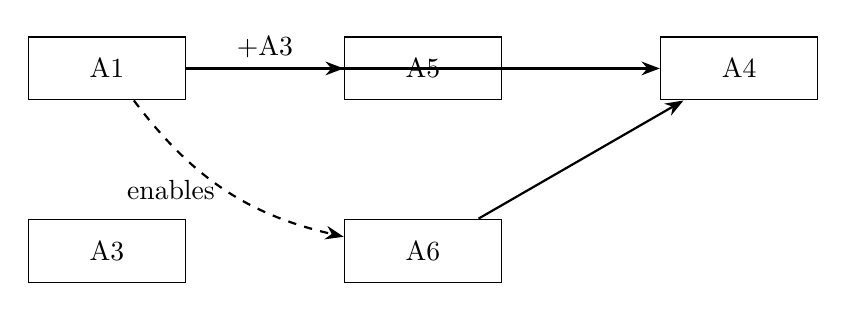
\begin{tikzpicture}[
    node distance=1.5cm,
    axiom/.style={rectangle, draw, minimum width=2cm, minimum height=0.8cm},
    arrow/.style={-{Stealth}, thick}
]
    \node[axiom] (A1) {A1};
    \node[axiom, right=2cm of A1] (A5) {A5};
    \node[axiom, below=of A1] (A3) {A3};
    \node[axiom, right=2cm of A5] (A4) {A4};
    \node[axiom, below=of A5] (A6) {A6};
    
    \draw[arrow] (A1) -- node[above] {+A3} (A5);
    \draw[arrow] (A1) -- (A4);
    \draw[arrow] (A6) -- (A4);
    \draw[arrow, dashed] (A1) to[bend right=20] node[left] {enables} (A6);
\end{tikzpicture}
\end{center}

\textbf{Key insight}: A1 is the root of the implication graph. Without A1, axioms A4--A6 cannot be meaningfully defined.

%==============================================================================
\section{Information-Theoretic Analysis}
\label{sec:information}
%==============================================================================

\subsection{Can Information Principles Derive Quantum Structure?}

We analyze whether information-theoretic principles can substitute for A1:

\begin{table}[ht]
\centering
\caption{Information principles by computation type}
\label{tab:info}
\begin{tabular}{lccc}
\toprule
Principle & Irreversible & Reversible & Quantum \\
\midrule
Information conservation & \texttimes & \checkmark & \checkmark \\
No-deleting & \texttimes & \checkmark & \checkmark \\
No-cloning & \texttimes & \texttimes & \checkmark \\
No-broadcasting & \checkmark & \checkmark & \checkmark \\
\bottomrule
\end{tabular}
\end{table}

\begin{theorem}[Information Conservation is Insufficient]
\label{thm:info-insufficient}
Information conservation does not imply quantum structure.
\end{theorem}

\begin{proof}
Reversible classical computation (Toffoli gates) conserves information but embeds in $\Sp(2N,\R)$, not $\SU(N)$. It satisfies A3 but not A1.
\end{proof}

\subsection{No-Cloning is a Consequence}

\begin{theorem}[No-Cloning Requires Superposition]
\label{thm:nocloning-requires}
The no-cloning theorem requires non-orthogonal states, which presuppose A1.
\end{theorem}

\begin{proof}
In classical computation, all pure states are orthogonal (standard basis vectors). Classical bits \emph{can} be cloned: measure and prepare. The no-cloning theorem is non-trivial only when non-orthogonal states exist, i.e., when A1 holds.
\end{proof}

\begin{remark}
This resolves a potential circular argument: one cannot derive A1 from no-cloning, because no-cloning presupposes A1.
\end{remark}

\subsection{Coherence Injection Experiment}

Using Resource Theory, we test whether classical operations can generate coherence:

\begin{proposition}[Classical Operations Cannot Generate Coherence]
\label{prop:coherence}
Permutation operations and dephasing are ``free operations'' that cannot increase coherence.
\end{proposition}

\begin{proof}
Let $C(\rho)$ be any valid coherence measure (e.g., $\ell_1$-norm of off-diagonals). For permutation $P$:
\[
C(P\rho P^\dagger) = C(\rho)
\]
since permutations merely relabel basis states. For dephasing $\mathcal{D}$:
\[
C(\mathcal{D}(\rho)) = 0 \leq C(\rho)
\]
Thus, classical operations preserve or destroy coherence, never amplify it.
\end{proof}

Experimental verification (Table~\ref{tab:coherence}) confirms this: injecting coherent states into classical computation results in coherence preservation (permutations) or destruction (dephasing), never amplification.

\begin{table}[ht]
\centering
\caption{Coherence under classical operations}
\label{tab:coherence}
\begin{tabular}{lccc}
\toprule
State & Operation & Initial $C$ & Final $C$ \\
\midrule
$|0\rangle$ & Identity & 0.0 & 0.0 \\
$|+\rangle$ & Identity & 1.0 & 1.0 \\
$|+\rangle$ & NOT & 1.0 & 1.0 \\
$|+\rangle$ & Dephasing & 1.0 & 0.0 \\
\bottomrule
\end{tabular}
\end{table}

%==============================================================================
\section{Universality Across Computation Models}
\label{sec:universality}
%==============================================================================

A critical question is whether our results are specific to SK combinatory logic or universal across computation models.

\subsection{Lambda Calculus Analysis}

Lambda calculus is computationally equivalent to SK combinatory logic (Church-Turing thesis). We verify it exhibits the same classical behavior.

\begin{theorem}[Lambda Calculus is Classical]
\label{thm:lambda}
Lambda calculus ($\beta$-reduction) is a classical computation model:
\begin{enumerate}
    \item $\beta$-reduction is deterministic (single-step choice doesn't affect normal form).
    \item State space is a simplex over term configurations.
    \item Cannot generate coherence.
\end{enumerate}
\end{theorem}

\begin{proof}
(1) Church-Rosser theorem guarantees confluence: all reduction paths converge to the same normal form (if it exists). This is classical determinism, not quantum superposition.

(2) The state space of $\lambda$-terms under reduction is discrete, forming a simplex $\Delta^{n-1}$ where $n$ is the number of reachable terms.

(3) $\beta$-reduction, when modeled as a transformation, acts as dephasing-like operation that destroys coherence rather than generating it.
\end{proof}

\begin{remark}[Church-Rosser $\neq$ Superposition]
The existence of multiple reduction paths in $\lambda$-calculus superficially resembles quantum superposition, but differs fundamentally:
\begin{itemize}
    \item \textbf{Church-Rosser}: Multiple paths represent \emph{choice} of reduction order; all paths converge.
    \item \textbf{Superposition}: Multiple states \emph{coexist} until measurement; interference occurs.
\end{itemize}
Confluence is classical non-determinism of choice, not quantum non-determinism of state.
\end{remark}

\begin{remark}[Probabilistic Computation]
\label{rem:probabilistic}
One might ask whether \emph{probabilistic} computation models (probabilistic Turing machines, probabilistic $\lambda$-calculus) could evade our conclusion. The answer is negative: probabilistic computation explores the \emph{interior} of the simplex $\Delta^{n-1}$ (mixed states over deterministic configurations), but does not extend the \emph{boundary} of the state space. The extreme points of a probabilistic classical system remain the deterministic pure states. In GPT terms, probabilistic computation corresponds to convex combinations within $\Omega$, not enlargement of $\Omega$ beyond the simplex. Thus, probabilistic computation satisfies neither A1 nor generates coherence---it remains classical.
\end{remark}

\subsection{SK $\leftrightarrow$ $\lambda$ Translation}

The standard translations confirm equivalence:
\begin{align}
    \mathbf{S} &= \lambda x.\lambda y.\lambda z. x\, z\, (y\, z) \\
    \mathbf{K} &= \lambda x.\lambda y. x \\
    \mathbf{I} &= \mathbf{S\, K\, K} = \lambda x. x
\end{align}

\subsection{Summary of Universality}

\begin{table}[ht]
\centering
\caption{Universality across computation models}
\label{tab:universality}
\begin{tabular}{lcccc}
\toprule
Model & Classical & Superposition & Coherence Gen. & A1 Required \\
\midrule
SK combinatory & \checkmark & \texttimes & \texttimes & \checkmark \\
RCA (Rule 90/150) & \checkmark & \texttimes & \texttimes & \checkmark \\
Toffoli/Fredkin & \checkmark & \texttimes & \texttimes & \checkmark \\
Lambda calculus & \checkmark & \texttimes & \texttimes & \checkmark \\
\midrule
Quantum circuits & \checkmark & \checkmark & \checkmark & (has A1) \\
\bottomrule
\end{tabular}
\end{table}

\begin{corollary}[Universal Result]
The requirement of A1 for quantum structure is independent of the choice of Turing-complete computation model.
\end{corollary}

%==============================================================================
\section{Discussion}
\label{sec:discussion}
%==============================================================================

\subsection{The Minimal Axiom Set}

Our analysis identifies the minimal axiom needed to ``upgrade'' classical computation to quantum mechanics:

\begin{center}
\fbox{\parbox{0.8\textwidth}{
\textbf{Minimal Quantum Axiom}: A1 (State Space Extension)

\medskip
The state space $\Omega$ extends beyond the simplex of probability distributions, allowing non-orthogonal pure states (superposition).
}}
\end{center}

All other quantum properties follow:
\begin{itemize}
    \item A5 (No-cloning): From A1 + A3
    \item A4 (Non-commutativity): Enabled by A1
    \item A6 (Contextuality): Enabled by A1
\end{itemize}

\subsection{What Computation Provides}

Classical computation naturally provides:
\begin{itemize}
    \item \textbf{A2 (Born rule)}: Linear probabilities are automatic in GPTs.
    \item \textbf{A3 (Reversibility)}: For reversible gates (Toffoli, Fredkin).
\end{itemize}

But computation \emph{cannot} provide A1. This is the ``quantum leap.''

\subsection{Quantization Diagram}

The relationship between computation, classical mechanics, and quantum mechanics is summarized in Figure~\ref{fig:quantization}.

\begin{figure}[ht]
\centering
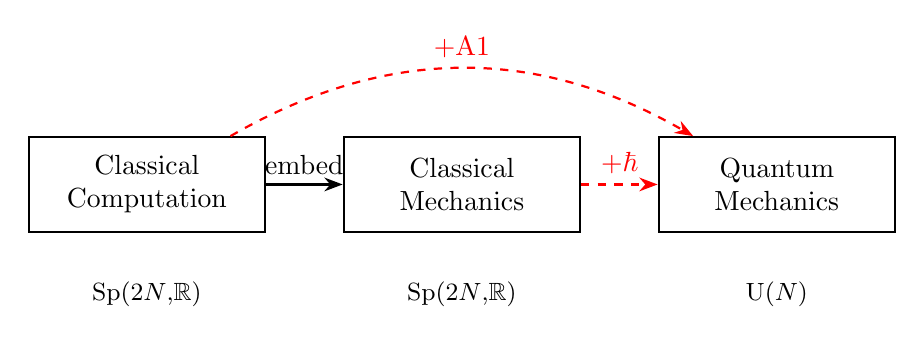
\begin{tikzpicture}[
    node distance=3cm,
    box/.style={rectangle, draw, thick, minimum width=3cm, minimum height=1.2cm, align=center},
    arrow/.style={-{Stealth}, thick}
]
    \node[box] (CC) at (-4,0) {Classical\\Computation};
    \node[box] (CM) at (0,0) {Classical\\Mechanics};
    \node[box] (QM) at (4,0) {Quantum\\Mechanics};
    
    \draw[arrow] (CC) -- node[above] {embed} (CM);
    \draw[arrow, dashed, red] (CM) -- node[above] {$+\hbar$} (QM);
    \draw[arrow, dashed, red] (CC) to[bend left=30] node[above] {$+$A1} (QM);
    
    \node[below=0.5cm of CC, font=\small] {Sp($2N$,$\R$)};
    \node[below=0.5cm of CM, font=\small] {Sp($2N$,$\R$)};
    \node[below=0.5cm of QM, font=\small] {U($N$)};
\end{tikzpicture}
\caption{Quantization paths. Computation embeds in classical mechanics (symplectic). The quantum leap requires either canonical quantization ($+\hbar$) or axiom A1 ($+$superposition).}
\label{fig:quantization}
\end{figure}

\subsection{The Role of Contextuality}

A1 enables contextuality (A6), but recent work suggests contextuality may be the key resource for quantum computational advantage~\cite{howard2014}. This raises an interesting question: \emph{If we take contextuality as the primitive axiom instead of A1, can we reconstruct full quantum mechanics?}

Our analysis suggests the answer is nuanced. Contextuality requires non-commuting observables (A4), which in turn requires non-orthogonal states---i.e., A1. Thus, contextuality presupposes A1 at the logical level. However, from a \emph{resource-theoretic} perspective, the relationship may be more subtle: A1 provides the ``raw material'' (superposition), while contextuality determines how this resource can be utilized computationally.

Whether contextuality alone (without explicitly postulating A1) can lead to the full Bloch ball structure remains an intriguing open question. If true, it would suggest that computational power, rather than state space geometry, is the more fundamental characterization of quantum mechanics.

\subsection{Implications}

\begin{enumerate}
    \item \textbf{For physics}: Quantum mechanics cannot be ``derived'' from computation; it must be \emph{postulated}.
    
    \item \textbf{For computer science}: The gap between classical and quantum computing is precisely A1---the ability to maintain superpositions.
    
    \item \textbf{For foundations}: Information-theoretic principles like no-cloning are downstream of superposition, not alternatives to it.
\end{enumerate}

%==============================================================================
\section{Conclusion}
\label{sec:conclusion}
%==============================================================================

We have systematically investigated the minimal axioms required to derive quantum structure from classical computation. Our main findings are:

\begin{enumerate}
    \item \textbf{A1 is the unique primitive axiom}: State space extension (superposition) cannot be derived from other axioms or from computation.
    
    \item \textbf{Information principles are consequences}: No-cloning, contextuality, and non-commutativity follow from A1; they cannot substitute for it.
    
    \item \textbf{Results are universal}: The same conclusions hold for SK combinatory logic, reversible cellular automata, Toffoli/Fredkin gates, and lambda calculus.
\end{enumerate}

The ``quantum leap'' from classical to quantum is precisely the addition of A1: the postulate that physical states can exist in superposition.

\subsection{Future Work}

\begin{itemize}
    \item \textbf{Formal verification}: Prove main theorems in Coq/Lean.
    \item \textbf{Physical interpretation}: What physical principle corresponds to A1?
    \item \textbf{Intermediate theories}: Are there GPTs between classical and quantum that satisfy A1 partially?
\end{itemize}

%==============================================================================
\section*{Acknowledgments}
%==============================================================================

The author thanks the reviewers for valuable feedback. All implementations are available at \url{https://github.com/future-apps-jp/omega/}.

%==============================================================================
\bibliographystyle{plain}
\begin{thebibliography}{99}

\bibitem{kohashiguchi2024sk}
H. Kohashiguchi,
``On the Independence of Quantum Structure from SK Combinatory Logic,''
arXiv preprint, 2024.

\bibitem{kohashiguchi2024limits}
H. Kohashiguchi,
``On the Limits of Deriving Quantum Structure from Reversible Computation: Symplectic Embedding of Reversible Gates and the Hierarchy of Quantum Resources,''
arXiv preprint, 2024.

\bibitem{chiribella2011}
G. Chiribella, G. M. D'Ariano, and P. Perinotti,
``Informational derivation of quantum theory,''
\emph{Physical Review A}, vol.~84, p.~012311, 2011.

\bibitem{hardy2001}
L. Hardy,
``Quantum theory from five reasonable axioms,''
arXiv:quant-ph/0101012, 2001.

\bibitem{masanes2011}
L. Masanes and M. P. M\"uller,
``A derivation of quantum theory from physical requirements,''
\emph{New Journal of Physics}, vol.~13, p.~063001, 2011.

\bibitem{streltsov2017}
A. Streltsov, G. Adesso, and M. B. Plenio,
``Colloquium: Quantum coherence as a resource,''
\emph{Reviews of Modern Physics}, vol.~89, p.~041003, 2017.

\bibitem{barrett2007}
J. Barrett,
``Information processing in generalized probabilistic theories,''
\emph{Physical Review A}, vol.~75, p.~032304, 2007.

\bibitem{chitambar2019}
E. Chitambar and G. Gour,
``Quantum resource theories,''
\emph{Reviews of Modern Physics}, vol.~91, p.~025001, 2019.

\bibitem{howard2014}
M. Howard, J. Wallman, V. Veitch, and J. Emerson,
``Contextuality supplies the `magic' for quantum computation,''
\emph{Nature}, vol.~510, pp.~351--355, 2014.

\end{thebibliography}

\end{document}

